% Autor: Leonhard Segger, Alexander Neuwirth
% Datum: 2017-10-30
\documentclass[
	% Papierformat
	a4paper,
	% Schriftgröße (beliebige Größen mit „fontsize=Xpt“)
	12pt,
	% Schreibt die Papiergröße korrekt ins Ausgabedokument
	pagesize,
	% Sprache für z.B. Babel
	ngerman
]{scrartcl}

% Achtung: Die Reihenfolge der Pakete kann (leider) wichtig sein!
% Insbesondere sollten (so wie hier) babel, fontenc und inputenc (in dieser
% Reihenfolge) als Erstes und hyperref und cleveref (Reihenfolge auch hier
% beachten) als Letztes geladen werden!

% Silbentrennung etc.; Sprache wird durch Option bei \documentclass festgelegt
\usepackage{babel}
% Verwendung der Zeichentabelle T1 (Sonderzeichen etc.)
\usepackage[T1]{fontenc}
% Legt die Zeichenkodierung der Eingabedatei fest, z.B. UTF-8
\usepackage[utf8]{inputenc}
% Schriftart
\usepackage{lmodern}
% Zusätzliche Sonderzeichen
\usepackage{textcomp}

% Mathepaket (intlimits: Grenzen über/unter Integralzeichen)
\usepackage[intlimits]{amsmath}
% Ermöglicht die Nutzung von \SI{Zahl}{Einheit} u.a.
\usepackage{siunitx}
% Zum flexiblen Einbinden von Grafiken (\includegraphics)
\usepackage{graphicx}
% Abbildungen im Fließtext
\usepackage{wrapfig}
% Abbildungen nebeneinander (subfigure, subtable)
\usepackage{subcaption}
% Funktionen für Anführungszeichen
\usepackage{csquotes}
% Zitieren, Bibliographie
\usepackage{biblatex}

% Verlinkt Textstellen im PDF-Dokument
\usepackage[unicode]{hyperref}
% "Schlaue" Referenzen (nach hyperref laden!)
\usepackage{cleveref}
% Zur Darstellung von Webadressen
\usepackage{url}
%chemische Formeln
\usepackage[version=4]{mhchem}
% siunitx: Deutsche Ausgabe, Messfehler getrennt mit ± ausgeben
\sisetup{
	locale=DE,
	separate-uncertainty
}
%\bibliography{6Mi_S2_25-10-2017_References}

\begin{document}
	
	\begin{titlepage}
		\centering
		{\scshape\LARGE Versuchsbericht zu \par}
		\vspace{1cm}
		{\scshape\huge E5 - Magnetische Suszeptibilität\par}
		\vspace{2.5cm}
		{\LARGE Gruppe 6Mi \par}
		\vspace{0.5cm}
		
		{\large Alexander Neuwirth (E-Mail: a\_neuw01@wwu.de) \par}
		{\large Leonhard Segger (E-Mail: l\_segg03@uni-muenster.de) \par}
		\vfill
		
		durchgeführt am 25.10.2017\par
		betreut von\par
		{\large Fabian Schöttke}
		
		\vfill
		
		{\large \today\par}
	\end{titlepage}
	\tableofcontents
	\newpage
	
	\section{Kurzfassung}
	Die Reaktion eines Stoffes auf ein Magnetfeld ist abhängig von der Volumensuszeptibilität $\xi_V$. Ist der Stoff diamagnetisch ($\xi_V<0$), so wird er vom Magneten schwach abgestoßen und ist er paramagnetisch ($\xi_V>0$), so wird sie schwach angezogen. Den Ferro- und Antiferromagnetismus haben wir in diesem Versuch nicht betrachtet.
	
	\section{Fermi Abschätzung zum Einfluss der Suszeptibilität auf die Oberfläche einer Flüssigkeit}
	\subsection{Methoden}
	Es ist zu erwarten, dass ein diamagnetischer Flüssigkeitsfilm über einem Magneten einen Berg ausbildet und ein paramagnetischer Flüssigkeitsfilm ein Tal ausbildet. 
	Um Rückschlüsse auf die Suszeptibilität von Flüssigkeiten zu untersuchen, wurde ein Laser auf eine Flüssigkeit in einer Petrischale gerichtet und die Reflexion des Lasers auf einer Wand beobachtet. Dann wurde vom Versuchsbetreuer unter der Petrischale ein Magnet hindurch bewegt. Aus der Änderung des Reflexionswinkels lässt sich dann die Höhe des Tal oder Berges über dem Magneten abschätzen. Untersucht wurde Wasser und mit Wasser verdünntes Manganchlorid.
	%TODO: Skizze mit Bezeichnungen aus dem Laborbuch
	\subsection{Ergebnisse}
	Bei Breite des Magneten $d \approx 1 \si{cm}$ , Ruhelage der Reflexion auf der Wand $b \approx 3 \si{m}$ und Abstand der Petrischale zur Wand $a \approx 6 \si{m}$ ergibt sich für die Auslenkung $\Delta y$ des Lasers auf der Wand: \newline
	$ \Delta y_\text{\ce{H2O}} \approx -7 \si{cm} \\
	\Delta y_\text{\ce{MnCl2}} \approx 15 \si{cm}$
	
	\begin{figure}[htb]
	  \centering
	    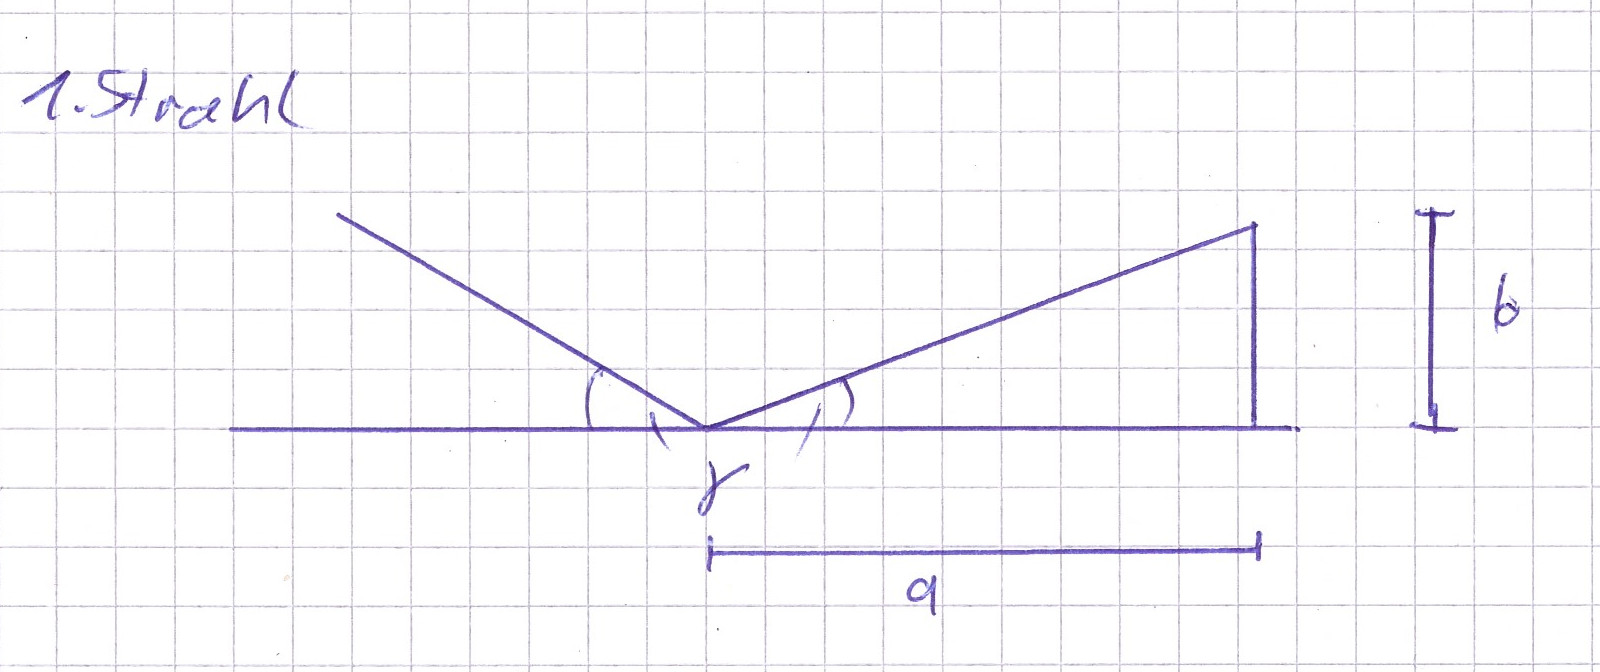
\includegraphics[width=0.6\textwidth]{Fermi1} 
	  \caption{Fermi Abschätzung Skizze Strahl 1}
	\end{figure}
		
	\begin{figure}[htb]
	  \centering
	    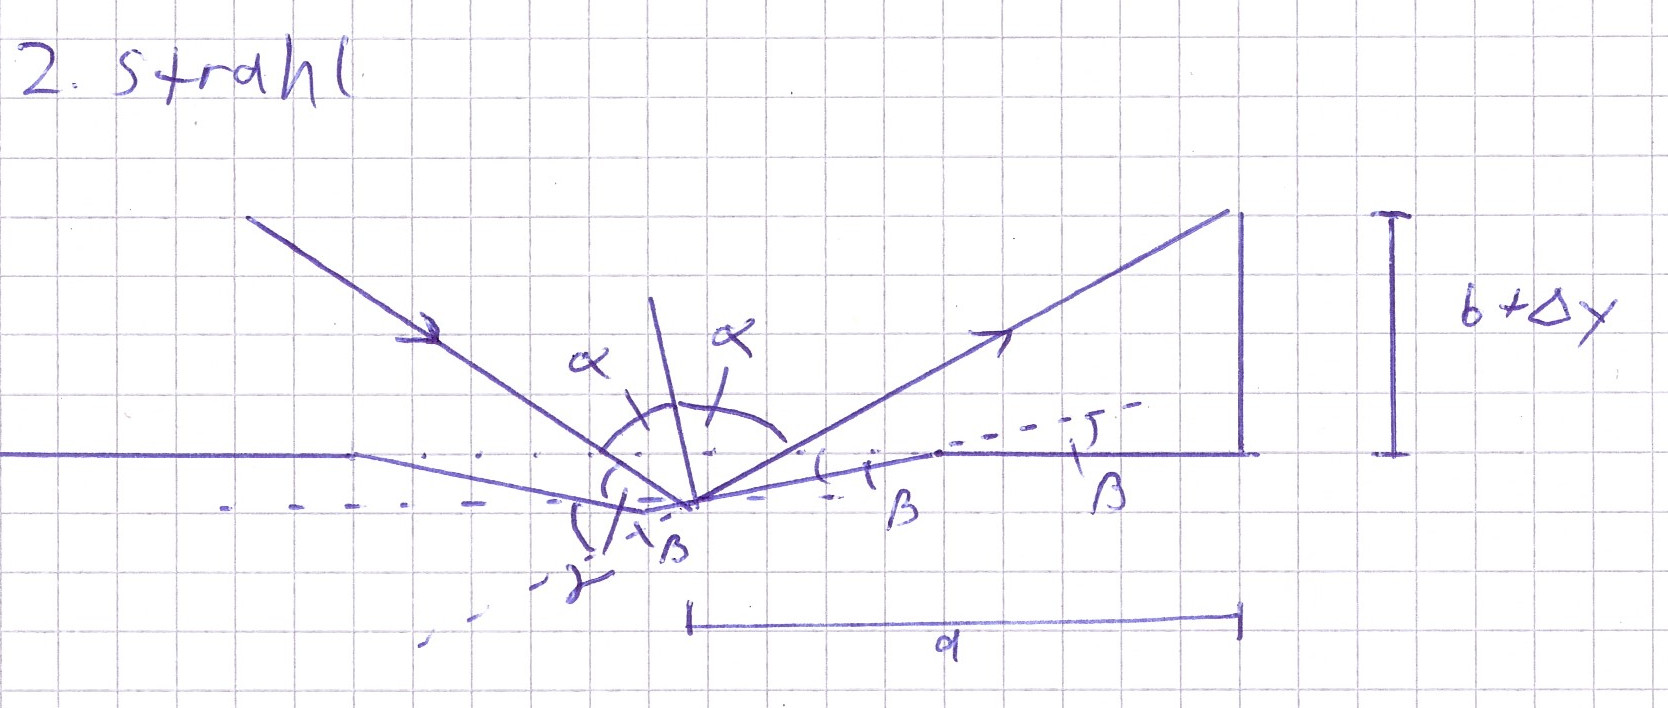
\includegraphics[width=0.6\textwidth]{Fermi2} 
	  \caption{Fermi Abschätzung Skizze Strahl 2}
	\end{figure}
	\begin{figure}[htb]
	  \centering
	    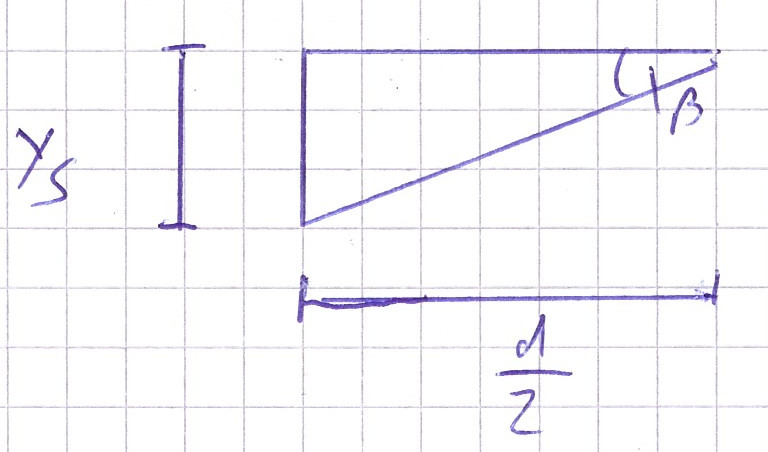
\includegraphics[width=0.6\textwidth]{Fermi3} 
	  \caption{Fermi Abschätzung Skizze Dreieck}
	\end{figure}

	\begin{gather*}
		\gamma = \arctan \left(\frac{b}{a}\right) \\
		\alpha = \ang{90} - \beta - \gamma \\
		\arctan \left(\frac{b+\Delta y}{a}\right) = \ang{180} - \gamma - 2\alpha \\
		\arctan \left(\frac{b+\Delta y}{a}\right) = \gamma + 2 \beta \\
		\arctan \left(\frac{b+\Delta y}{a}\right) =   \arctan \left(\frac{b}{a}\right) + 2 \beta \\
		\Rightarrow \beta = \frac{\arctan \left(\frac{b+\Delta y}{a}\right) -  \arctan \left(\frac{b}{a}\right)}{2} \\
		\Rightarrow y_\text{S} = \tan (\beta) \frac{d}{2}  \\
	\end{gather*}
	Setzt man die gemessenen Werte in die Formel ein so erhält man: $ y_{\text{S,\ce{H2O}}} = \SI{-0,0023}{ cm} $ und $y_{\text{S,\ce{MnCl2}}} = \SI{0,00495}{ cm} $. Das Wasser wird folglich abgestoßen und die Mangan-Chlorid-Lösung wird von dem Magneten angezogen.
	\subsubsection*{Unsicherheiten}
	Beim Aufstellen der Gleichung wurde die Approximatation verwendet, dass beide Reflektionen in gleichem Abstand zur Wand stattfinden. Dass dies kaum Einfluss auf das Ergebniss nimmt zeigt die folgende Rechnung:
	\begin{align*}
		\Delta x &= \tan (\gamma) y_\text{S} \\
		\Delta x &= \frac{b}{a} y_\text{S}
	\end{align*}
	Da unsere Schätzung von $a$, bzw. von dem Verhältnis $\frac{b}{a}$, eine größere Unsicherheit aufweißt, als der Fehler $\Delta x$, der bei der Näherung entsteht, ist dieser vernachlässigbar.



	\subsection{Schlussfolgerung}
	Zur Näherung der Verformung der Wasseroberfläche nutzen wir eine Fermi-Abschätzung. Dafür treffen wir die vereinfachende Annahme, dass der Berg bzw. das Tal eine Dreiecksform haben mit dem Ziel, die Höhe $h$ des Dreiecks zu bestimmen. Zugrunde legen wir das Reflexionsgesetz für die Reflexion des Lasers an der Tal-/Bergwand.
	
	\section{Bestimmung der Volumensuszeptibilität von Glas, Kohlenstoff und Graphit}
	\subsection{Methoden}
	Um die Volumensuszeptibilität von Glas, Graphit und Aluminium zu bestimmen, haben wir die Änderung der Belastung einer Waage, auf der die Probe platziert wurde, mit und ohne Magneten darüber gemessen. Der Magnet war ein Neodymmagnet, der an einem Stativarm befestigt ist und daran über die Waage und zurück geschwenkt werden konnte. Dabei haben wir zunächst mit der Probe die Höhe des Magneten eingestellt und dann die Waage auf Null gesetzt während der Magnet über die Probe geschwenkt war. Dann haben wir den Magneten in die maximal von der Probe entfernte Position gebracht und die Änderung der auf der Waage angezeigten Masse notiert. Es wurde jeweils der negative Wert der Anzeige notiert, da wir die Änderung der Belastung von der Ruhelage zur Lage mit Einfluss des Magneten messen wollten. Dieses Vorgehen minimiert die Anzahl der nötigen Schwenkvorgänge, die die Messung beeinflussen könnten. Dann haben wir dieselbe Messung mit dem leeren Probenhalter (Dummy) vorgenommen, ohne die Höhe des Magneten zu ändern. Dies ermöglicht es uns den Einfluss des Probenhalters auf die Messung zu subtrahieren. Dieses Vorgehen haben wir für alle drei Proben wiederholt. Da wir zunächst den Abstand $d$ zwischen Probe und Magnet nicht ausreichend präzise eingestellt hatten, habe wir die Messung wiederholt, wobei wir darauf geachtet haben, dass beim Einstellen des Abstands mit einem \SI{1}{\milli \meter} dicken Kunststoffstück, keine mechanische Kraft vom Stativarm auf die Waage ausgeübt wird. Die Stärke des Neodymmagneten wird als $B_r = (1,87 \pm 0,1 ) \si{\tesla}$ angegeben.
	\subsection{Ergebnisse und Diskussion}
	Die Abmessungen des zylinderförmigen Magneten können exakt als $R_\text{neo}=30 \si{mm}$ und $D_\text{neo}=15 \si{mm}$ angenommen werden. Ebenfalls als exakt nehmen wir den Abstand zwischen Magnet und Probe $d=1\si{mm}$ und den Ortsfaktor $g=9,81\si{\meter \per \second \squared}$ an. 
	\newline
	Ergebnisse der Messung der Änderung der effektiven Masse $\Delta m$ : \newline
	\begin{tabular}{ r | c | c | c | c | c | c |}
		 & Glas & Glasdummy & Graphit & Graphitdummy & Aluminium & Aluminiumdummy\\ \hline
		$\Delta m  \si{/g}$ & 0,35 &0,33 &1,79 & 0,35 & 0,30 & 0,36\\
	\end{tabular}
	%TODO Abmessungen Proben

	\subsection{Schlussfolgerung}
	Für die Bestimmung der Volumensuszeptibilität nutzen wir die Gleichung
	\begin{equation}
	\label{Suzeptibilitaet}
	\Xi=\frac{2 \mu_0 g \cdot \Delta m}{V_s(\partial B_z^2 /\partial z)}.
	\end{equation}
	Das Magnetfeld $B(x)$ eines Zylindermagneteten im Abstand z auf der Achse des Zylinders ist angegeben als
	\begin{equation}
	\label{Magnetfeld_Zylinder}
	B(z)=\frac{B_r}{2}\left( \frac{D+z}{\sqrt{R^2+(D+z)^2}}-\frac{z}{\sqrt{R^2 +z^2}}\right).
	\end{equation}
	Dabei kann $\partial B_z^2 /\partial z$ genähert werden durch 
	\begin{equation}
	\label{Ableitung_Magnetfeld}
	\partial B_z^2 /\partial z \approx \frac{B_z^2(d) - B_z^2(d+h_s)}{h_s}.
	\end{equation}
	%TODO not sure, ob das eher zu Diskuss-Ion zählt
	
	\section{Untersuchung der gegenseitigen Reaktion von Magneten und Aluminium bei Relativbewegung}
	\subsection{Methoden}
	\paragraph{Magnetstab und Aluminiumplättchen}
	Wir haben die Reaktion eines Aluminiumplättchen (an langem Faden aufgehängt) auf die Bewegung eines Magnetstabs (drei Würfelmagneten) beobachtet. Dafür bewegten wir den Magneten senkrecht auf das Plättchen zu sowie parallel an ihm vorbei.
	Danach wurde die selbe Untersuchung für einen Aluminiumkamm durchgeführt. Aluminium wurde hierbei für die als Versuchsobjekt gewählt, weil es den elektrischen Strom leitet und gleichzeitig nicht ferromagnetisch ist. Dies wäre auch z.B. bei Kupfer der Fall, aber Aluminium ist deutlich günstiger. %Ist bissl useless die Preisbemerkung, kann nach Belieben gelöscht werden
	\paragraph{Aluminiumröhre und Permanentmagnet}
	Wir ließen einen Permanentmagneten durch ein Aluminiumrohr fallen. Dieser Versuch wurde dann mit einem Aluminiumrohr, das der Länge nach aufgeschnitten ist, wiederholt.
	\subsection{Ergebnisse}
	\paragraph{Magnetstab und Aluminiumplättchen}
	Wenn der Magnetstab auf das Plättchen zubewegt wird, bewegt sich das aufgehängte Plättchen davon weg. Wenn sich andersherum der Magnetstab vom Aluminiumplättchen entfernt, folgt das Plättchen dieser Bewegung. Sobald die Bewegung gestoppt wird, kehrt das Plättchen auch in seinen Ausgangszustand zurück. Eine Bewegung parallel zur Oberfläche, lässt das Plättchen dem Magneten folgen. Beide Effekte erlauben nur eine Auslenkung bis zu einem Winkel, der mit der Bewegungsgeschwindigkeit wächst. %Zu oft "Bewegung"
	Beim Aluminiumkamm, sind die beschriebenen Effekte nur noch stark abgeschwächt beobachtbar.
	\paragraph{Aluminiumröhre und Permanentmagnet}
	Im Vollrohr fällt der Magnet deutlich langsamer, als er es in Luftumgebung tut. Im aufgeschnittenen Rohr wird dieser Effekt ebenfalls noch beobachtet, ist aber deutlich abgeschwächt.
	\subsection{Schlussfolgerung}
	In beiden Fällen sind Wirbelströme die Ursache des beobachteten Phänomens.
	Die Bewegung des Magnetstabes ruft eine Änderung des Magnetfeldes durch das Aluminiumplättchen hervor. Dies ruft nach dem Faraday'schen Induktionsgesetz $U_\text{ind}= - \frac{\text{d}}{\text{d}t} \int \vec{V} \text{d} \vec{A}$ eine Potentialdifferenz hervor, die zu einem Wirbelstrom in dem Aluminiumplättchen führt. Dieser Wirbelstrom ist nach der Lenz'schen Regel immer so gerichtet, dass sein Magnetfeld der Ursache, also der Änderung des Magnetfeldes des Magnetstabes, entgegen gerichtet ist.%muss man die ausformulieren?
	Die zueinander gerichteten Magnetfelder bei der Weg-Bewegung des Magnetstabes verursachen die beobachtete Anziehung des Plättchens und die entgegengesetzt gerichteten Magnetfelder bei der Hin-Bewegung die Abstoßung.
	Im Aluminiumkamm sind die Wirbelströme nur noch innerhalb der Zinken und nicht mehr über die gesamten Fläche möglich. Dies verursacht den stark verringerten Effekt des Magnetstabes. \par
	Ähnlich verhält es sich mit dem fallenden Magneten im Aluminiumrohr. Die Änderung des Magnetfeldes durch den Querschnitt des Rohres verursacht Wirbelströme in diesem, die ein Magnetfeld induzieren, welches über dem fallenden Magneten dessen Magnetfeld in der Richtung entspricht und unter ihm dessen Magnetfeld entgegengesetzt ist. Diese Magnetfelder bremsen den Fall des Magneten. Im aufgeschnittenen Rohr können die Wirbelströme nicht mehr im Querschnitt stattfinden, sondern nur noch auf der gesamten Mantelfläche, weshalb der bremsende Effekt deutlich kleiner ist. %Ist das true und vor allem, kann man das deutlicher sagen?
	%TODO Skizze aus Internet? 
	%\printbibliography
\end{document}
